\section{Results}
\label{sec:results}

Seven of the eight runs pass both validity gates. Qwen3-8B cut off 4.0\% of its answers at the token limit, so its numbers are descriptive only.

\subsection{Only large reasoning models respond to the horizon}

Figure~\ref{fig:use} shows, for each model, how often its answer is a best eight-decision move on sensitive states, next to its H-blind baseline. For six of the eight models the two numbers coincide. Telling them to look eight decisions ahead does not move their answers toward the long-horizon move. This holds at every horizon we tested (Appendix~\ref{app:curves}). Qwen3-32B and gpt-oss-120b are the exceptions. On both characters, their $H{=}8$ answers hit the long-horizon move far more often than their own $H{=}1$ answers do. For gpt-oss the rates are .36 against .25 (Ironclad) and .31 against .21 (Silent). For Qwen3-32B they are .28 against .22 and .30 against .19. McNemar's test gives $p \le .026$ in all four cases.

Size alone does not produce this. Llama-3.3-70B has more than twice the parameters of Qwen3-32B and no explicit reasoning, and its use rate sits at its baseline on both characters. Within one family the effect grows with scale: Qwen3-8B does not respond, Qwen3-14B moves slightly but stays within its baseline, and Qwen3-32B responds clearly.

\begin{figure}[t]
\centering
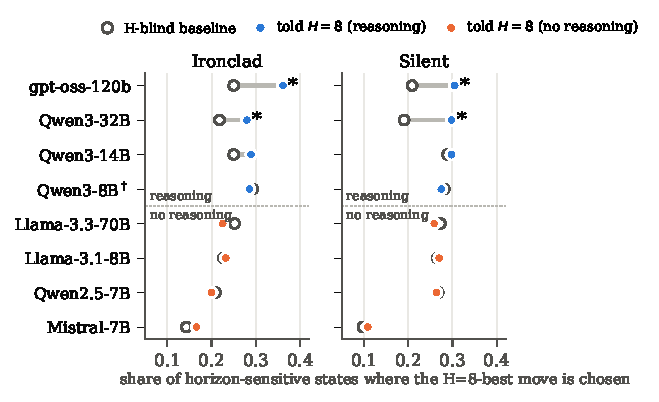
\includegraphics[width=\columnwidth]{figures/use_vs_baseline.pdf}
\caption{How often each model picks the best eight-decision move on sensitive states when told $H{=}8$ (filled), against its H-blind baseline (open), which is its own $H{=}1$ answer judged by the same standard. A model that ignores $H$ sits on its baseline. $^*$McNemar $p<.05$. $^\dagger$Failed the truncation gate, so descriptive only.}
\label{fig:use}
\end{figure}

\subsection{Responding is not planning}

The primary statistic tells a more sobering story (Table~\ref{tab:primary}). Five models show no effect, with confidence intervals tight around zero. The three models that move their answers, Qwen3-14B, Qwen3-32B and gpt-oss-120b, show a positive difference on Ironclad and, for gpt-oss, on Silent. In every case the difference comes from the control side. Their gain on sensitive states is close to zero, while their score on control states \emph{falls} when told to look further ahead. The instruction makes them abandon moves that were already right.

Figure~\ref{fig:decomp} shows where the answers go (a post hoc breakdown). When gpt-oss is told $H{=}8$, it gives up the greedy move on 314 of the 880 sensitive states, yet only 91 of those switches land on a best long-horizon move. The rest go to other moves, which on average score no better than the greedy move they replaced. Qwen3-32B behaves the same way: 73 of 209 switches find the long-horizon move. On control states, both models drop between a fifth and a third of their correct answers. The instruction works as a cue to avoid the obvious move. It does not lead the models to the move that looking ahead would reveal.

The state in Figure~\ref{fig:example} shows the pattern in a single case. At $H{=}1$, gpt-oss plays Pommel Strike, the best move, and explains that it ``deals the most damage this turn.'' At $H{=}8$ it switches to Feel No Pain, a card that grants block whenever a card is later exhausted, reasoning that it ``sets up future block generation.'' The switch sounds like planning, but the move is worth .53 on the eight-decision scale. Bash, which keeps the boss Vulnerable, is worth 1. Qwen3-32B plays Bash at both horizons.

\begin{table}[t]
\centering
\footnotesize
\setlength{\tabcolsep}{2pt}
\begin{tabular}{@{}lrr@{}}
\toprule
Model & Ironclad & Silent \\
\midrule
Mistral-7B & $+.013$ {\scriptsize$[-.03,+.06]$} & $+.033$ {\scriptsize$[-.01,+.08]$} \\
Qwen2.5-7B & $-.001$ {\scriptsize$[-.01,+.01]$} & $-.014$ {\scriptsize$[-.03,+.00]$} \\
Llama-3.1-8B & $+.003$ {\scriptsize$[-.01,+.01]$} & $-.000$ {\scriptsize$[-.01,+.01]$} \\
Llama-3.3-70B & $+.016$ {\scriptsize$[-.03,+.06]$} & $+.001$ {\scriptsize$[-.04,+.04]$} \\
Qwen3-8B$^\dagger$ & $-.031$ {\scriptsize$[-.10,+.03]$} & $+.018$ {\scriptsize$[-.04,+.07]$} \\
Qwen3-14B & $\mathbf{+.100}$ {\scriptsize$[+.04,+.16]$} & $+.005$ {\scriptsize$[-.04,+.05]$} \\
Qwen3-32B & $\mathbf{+.125}$ {\scriptsize$[+.07,+.18]$} & $+.045$ {\scriptsize$[-.01,+.10]$} \\
gpt-oss-120b & $\mathbf{+.155}$ {\scriptsize$[+.09,+.22]$} & $\mathbf{+.074}$ {\scriptsize$[+.02,+.13]$} \\
\midrule
\multicolumn{3}{@{}l}{\footnotesize Of which, gain on sensitive / control states:} \\
gpt-oss-120b & $+.014 \,/\, {-.142}$ & $-.032 \,/\, {-.107}$ \\
\bottomrule
\end{tabular}
\caption{Primary statistic: gain from the $H{=}8$ instruction on sensitive states minus gain on control states, with 95\% bootstrap intervals. Bold: rejects zero at $\alpha=.025$. The lower row shows that the positive values come from losses on control states.}
\label{tab:primary}
\end{table}

\begin{figure}[t]
\centering
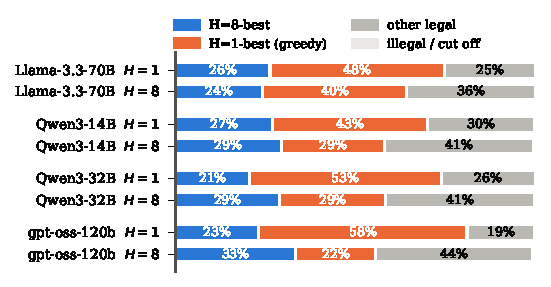
\includegraphics[width=\columnwidth]{figures/decomposition.pdf}
\caption{What models answer on sensitive states (both characters, 880 states) at $H{=}1$ and $H{=}8$. Responsive models move answers out of the greedy class, but mostly into other non-best moves. Post hoc.}
\label{fig:decomp}
\end{figure}

\subsection{It is not about knowing the game}

Our prompts name each card without describing it, so a model must recall what ``Bash'' does. A reviewer could fairly ask whether the horizon results reflect gaps in game knowledge, or recognition of famous card names, rather than planning. We tested both explanations in a pre-registered amendment on the 1,169 states that hold no targeted skill card (see Limitations). In the \emph{described} condition, every prompt carries an exact rulebook generated from the simulator: what each visible card does, how each enemy behaves and how every effect works. In the \emph{renamed} condition, every card, enemy and relic name, and the name of the game, is replaced by a neutral code such as ``Card K7''. We ran both conditions on one model that ignores the horizon (Llama-3.1-8B) and one that responds to it (gpt-oss-120b).

None of the eight pre-registered contrasts survives Holm correction \citep{holm1979} (Table~\ref{tab:knowledge}). With the rulebook, Llama-3.1-8B still ignores the horizon, with intervals of about $\pm.02$. Its blind spot is not a knowledge gap. gpt-oss plays somewhat better overall with the rulebook (mean $H{=}8$ quality rises from .71 to .76), but its use of the horizon does not change reliably. With all names hidden it still responds to the horizon at the same rate, so recognizing famous cards is not what drives it.\footnote{gpt-oss cut off 1.9\% of its renamed-condition answers, above the 1\% gate, so its familiarity contrasts are descriptive.}

\begin{table}[t]
\centering
\footnotesize
\setlength{\tabcolsep}{1.5pt}
\begin{tabular}{@{}llrr@{}}
\toprule
& & Knowledge & Familiarity \\
Model & Char. & {\scriptsize described $-$ base} & {\scriptsize renamed $-$ described} \\
\midrule
Llama-3.1-8B & IC & $-.003$ {\scriptsize$[-.02,+.02]$} & $+.017$ {\scriptsize$[-.02,+.05]$} \\
 & Silent & $-.000$ {\scriptsize$[-.02,+.02]$} & $-.005$ {\scriptsize$[-.04,+.03]$} \\
gpt-oss-120b & IC & $+.073$ {\scriptsize$[-.00,+.15]$} & $+.081^\dagger$ {\scriptsize$[-.00,+.16]$} \\
 & Silent & $+.073$ {\scriptsize$[-.01,+.15]$} & $+.084^\dagger$ {\scriptsize$[+.01,+.16]$} \\
\bottomrule
\end{tabular}
\caption{Knowledge and familiarity contrasts: change in the primary statistic between conditions, paired by state, 95\% intervals. None rejects after Holm correction over all eight. $^\dagger$Descriptive (gate failed).}
\label{tab:knowledge}
\end{table}

\subsection{Robustness}

Every conclusion above holds when any one of the five encounters is removed, and when the 591 states affected by the oracle limitation described under Limitations are removed (Appendix~\ref{app:robust}). A prompt variant that defines ``decision transition'' explicitly changes nothing for either model tested (Appendix~\ref{app:amendments}). The full-game scores of these models from an earlier version of the benchmark do not predict their horizon use. Those scores sit at a ceiling for combat and a floor for full runs, which is exactly why a controlled test is needed.
